\documentclass[11pt,a4paper]{article}
\usepackage[czech]{babel}
\usepackage[utf8]{inputenc}
\usepackage[T1]{fontenc}
\usepackage[top=3cm, left=2cm, text={17cm, 24cm}]{geometry}
\usepackage{graphicx}
\usepackage{amsmath}
\usepackage{multirow}
\usepackage[bookmarksopen,colorlinks,plainpages=false,urlcolor=blue,unicode]{hyperref}
\usepackage{url}
\usepackage{listings}

\newcommand{\minitab}[2][l]{\begin{tabular}{#1}#2\end{tabular}}
\newcommand{\sub}[1]{\ensuremath{_{\textnormal{#1}}}}
\newcommand{\bi}[1]{\textit{\textbf{#1}}}


\begin{document}


\def\author{Pavel Frýz}
\def\email{xfryzp00@stud.fit.vutbr.cz}
\def\projname{Woo Lam $\Pi^f$}
\begin{titlepage}

% \vspace*{1cm}
\begin{figure}[!h]
  \centering
  
\includegraphics[height=5cm]{logo}
\end{figure}

\vfill

\begin{center}
\begin{Large}
Dokumentace k~projektu z~předmětu IMS\\
\end{Large}
\bigskip
\begin{Huge}
\projname\\
\end{Huge}
\end{center}

\vfill

\begin{center}
\begin{Large}
\today
\end{Large}
\end{center}

\vfill

\begin{flushleft}
\begin{large}
\begin{tabular}{ll}
Autor: & \authorv, \url{\emailv} \\
 & \authorf, \url{\emailf} \\
 & Fakulta informačních technologií \\
 & Vysoké učení technické v~Brně \\
\end{tabular}
\end{large}
\end{flushleft}
\end{titlepage}


\section{Popis protokolu}
Protokol vytvořil profesor Texaské univerzity v Austinu Simon S.\,Lam
a jeho bývalý student Thomas Y. C. Woo. Protokol $\Pi^f$ byl představen
v \cite{wl94}. Protokol provádí pouze jednosměrnou autentizaci, autentizuje
účastníka A vůči B. Autentizace probíhá na důvěryhodném serveru(S), který
sdílí klíč s každým účastníkem, protokol používá symetrickou kryptografii.
Komunikici zahujeje subjekt A, subjekt B poté vygeneruje nonce a pošle ho A.
A zašifruje nonce, společně s identifikátory subjektů a vše pošle zpět B, který
k tomu přidá téže informace a vše zašifruje. Poté autentizační server ověří obě
zašifrované zprávy a provede překlad klíčů, zprávu zašifrovanou A dešifruje a znovu ji
zašifruje klíčem sdíleným z B. Toto pak pošle B, který ověří nonce. Pokud B dokončí
provádění protokolu, tak iniciátor spojení je subjekt A deklarovaný v první zprávě.
Z protokolu $\Pi^f$ jsou postupným zjednodušováním odvozeny protokoly $\Pi^1$, $\Pi^2$,
$\Pi^3$ a $\Pi$, ale zatímco protokol $\Pi^f$ je korektní, jeho zjednodušené verze jsou
nachýlné proti podvržení identity \cite{cj97}.

\begin{figure}[htb]
  \centering
  \begin{tabular}{ll}
  \textbf{Textová reprezentace \cite{repr}:}& \textbf{Grafická reprezentace:}\\
  \begin{minipage}[c]{0.49\textwidth}
    \begin{tabular}{ll}
    $A,B,S\colon$ & Subjekty\\
    $K_{AS},K_{BS}\colon$ & Sdílené klíče\\
    $N_B\colon$ & Nonce
    \end{tabular}
    \begin{enumerate}
    \item $A \rightarrow B\colon A$
    \item $B \rightarrow A\colon N_B$
    \item $A \rightarrow B\colon \{A,B,N_B\}_{K_{AS}}$
    \item $B \rightarrow S\colon \{A,B,N_B, \{A,B,N_B\}_{K_{AS}}\}_{K_{BS}}$
    \item $S \rightarrow B\colon \{A,B,N_B\}_{K_{BS}}$
    \end{enumerate}
  \end{minipage}
  &
  \begin{minipage}[c]{0.49\textwidth}
    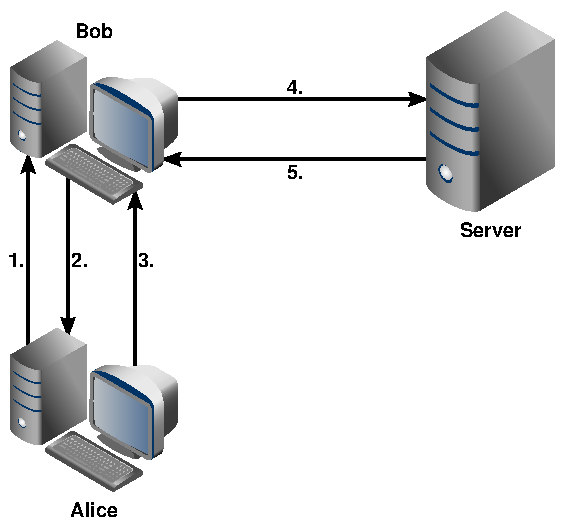
\includegraphics[width=0.85\textwidth]{net}
  \end{minipage}
  \end{tabular}
\end{figure}

\section{Analýza protokolu}
Počáteční, zakázané a cílové znalosti a předpokladý jsou uvedeny v tabulce \ref{tab1}.
Znalost subjektu A je označena \textbf{A:}, následované listem znalostí. Předpoklady subjektu
A o znalostech B jsou označeny \textbf{A:B:}. Znalosti a předpoklady po jedtlivích krocích jsou
uvedeny v tabulce \ref{tab2}. Nové znalosti a přepoklady jsou označeny \bi{takto}.
\bigskip
\begin{table}[htb]
  \footnotesize
  \catcode`\-=12
  \centering
  \begin{tabular}{|c|l|l|} \hline \label{tab1}
  \textbf{Krok} & \textbf{Znalosti} & \textbf{Předpoklady}\\\hline
  \multirow{3}{*}{\minitab[c]{Počáteční\\podmínky}}
    &\textbf{A:} A, B, S, K\sub{AS}                       %pocatecni znalosti A
    &\textbf{A:B:} \textbf{A:S:} K\sub{AS}\\            %pocatecni predpoklady A
    &\textbf{B:} B, S, N\sub{B}, K\sub{BS}                %pocatecni znalosti B
    &\textbf{B:A:} \textbf{B:S:} K\sub{BS}\\            %pocatecni predpoklady B
    &\textbf{S:} A, B, S, K\sub{AS}, K\sub{BS}             %pocatecni znalosti S
    &\textbf{S:A:} K\sub{AS} \textbf{S:B:} K\sub{BS}\\  %pocatecni predpoklady S
    \hline
  \multirow{3}{*}{\minitab[c]{Cílové\\podmínky}}
    & \textbf{A:} N\sub{B}   %cilove znalosti A
    &\\ %cilove predpoklady A
    &   %cilove znalosti B
    &\textbf{B:A:} N\sub{B} \textbf{B:S:} N\sub{B} \\ %cilove predpoklady B
    &   %cilove znalosti S
    &\textbf{S:A:} N\sub{B} \textbf{S:B:} N\sub{B}\\ %cilove predpoklady S
    \hline
  \multirow{3}{*}{\minitab[c]{Zakázané\\cílové\\podmínky}}
    &\textbf{A:} K\sub{BS}&\\
    &\textbf{B:} K\sub{AS}&\\&&\\
    \hline
  \end{tabular}
  \caption{Počáteční, zakázané a cílové znalosti a předpoklady}
\end{table}
\newpage
\begin{table}[htb]
  \footnotesize
  \catcode`\-=12
  \centering
  \begin{tabular}{|c|l|l|} \hline \label{tab2}
  \multirow{3}{*}{1}
    &\textbf{A:} A, B, S, K\sub{AS}
    &\textbf{A:B:} \bi{A}
     \textbf{A:S:} K\sub{AS} \\
    &\textbf{B:} \bi{A}, B, S, N\sub{B}, K\sub{BS}
    &\textbf{B:A:} \bi{A}
     \textbf{B:S:} K\sub{BS} \\
    &\textbf{S:} A, B, S, K\sub{AS}, K\sub{BS}
    &\textbf{S:A:} K\sub{AS}
     \textbf{S:B:} K\sub{BS} \\
    \hline
  \multirow{3}{*}{2}
    &\textbf{A:} A, B, S, \bi{N\sub{\bi{B}}}, K\sub{AS}
    &\textbf{A:B:} A, \bi{N\sub{\bi{B}}}
     \textbf{A:S:} K\sub{AS} \\
    &\textbf{B:} A, B, S, N\sub{B}, K\sub{BS}
    &\textbf{B:A:} A, \bi{N\sub{\bi{B}}}
     \textbf{B:S:} K\sub{BS} \\
    &\textbf{S:} A, B, S, K\sub{AS}, K\sub{BS}
    &\textbf{S:A:} K\sub{AS}
     \textbf{S:B:} K\sub{BS} \\
    \hline
  \multirow{3}{*}{3}
    &\textbf{A:} A, B, S, N\sub{B}, K\sub{AS}
    &\textbf{A:B:} A, N\sub{B}, \bi{\{A, B, N\sub{\bi{B}}\}\sub{\bi{K\sub{\bi{AS}}}}}
     \textbf{A:S:} K\sub{AS} \\
    &\textbf{B:} A, B, S, N\sub{B}, K\sub{BS}, \bi{\{A, B, N\sub{\bi{B}}\}\sub{\bi{K\sub{\bi{AS}}}}}
    &\textbf{B:A:} A, N\sub{B}, \bi{\{A, B, N\sub{\bi{B}}\}\sub{\bi{K\sub{\bi{AS}}}}}
     \textbf{B:S:} K\sub{BS} \\
    &\textbf{S:} A, B, S, K\sub{AS}, K\sub{BS}
    &\textbf{S:A:} K\sub{AS}
     \textbf{S:B:} K\sub{BS} \\
    \hline
  \multirow{3}{*}{4}
    &\textbf{A:} A, B, S, N\sub{B}, K\sub{AS}
    &\textbf{A:B:} A, N\sub{B}, \{A, B, N\sub{B}\}\sub{K\sub{AS}}
     \textbf{A:S:} K\sub{AS} \\
    &\textbf{B:} A, B, S, N\sub{B}, K\sub{BS}, \{A, B, N\sub{B}\}\sub{K\sub{AS}}
    &\shortstack[l]{\textbf{B:A:} A, N\sub{B}, \{A, B, N\sub{B}\}\sub{K\sub{AS}}\\
     \textbf{B:S:} \bi{A}, \bi{B}, \bi{N\sub{\bi{B}}}, K\sub{BS}, \bi{\{A, B, N\sub{\bi{B}}\}\sub{\bi{K\sub{\bi{AS}}}}}} \\
    &\textbf{S:} A, B, S, \bi{N\sub{\bi{B}}}, K\sub{AS}, K\sub{BS}
    &\shortstack[l]{\textbf{S:A:} \bi{A}, \bi{B}, \bi{N\sub{\bi{B}}}, K\sub{AS}\\
     \textbf{S:B:} \bi{A}, \bi{B}, \bi{N\sub{\bi{B}}}, K\sub{BS}, \bi{\{A, B, N\sub{\bi{B}}\}\sub{\bi{K\sub{\bi{AS}}}}}} \\
    \hline
  \multirow{3}{*}{5}
    &\textbf{A:} A, B, S, N\sub{B}, K\sub{AS}
    &\textbf{A:B:} A, N\sub{B}, \{A, B, N\sub{B}\}\sub{K\sub{AS}}
     \textbf{A:S:} K\sub{AS} \\
    &\textbf{B:} A, B, S, N\sub{B}, K\sub{BS}, \{A, B, N\sub{B}\}\sub{K\sub{AS}}
    &\shortstack[l]{\textbf{B:A:} A, N\sub{B}, \{A, B, N\sub{B}\}\sub{K\sub{AS}}\\
     \textbf{B:S:} A, B, N\sub{B}, K\sub{BS}, \{A, B, N\sub{B}\}\sub{K\sub{AS}}} \\
    &\textbf{S:} A, B, S, N\sub{B}, K\sub{AS}, K\sub{BS}
    &\shortstack[l]{\textbf{S:A:} A, B, N\sub{B}, K\sub{AS}\\
     \textbf{S:B:} A, B, N\sub{B}, K\sub{BS}, \{A, B, N\sub{B}\}\sub{K\sub{AS}}} \\
    \hline
  \end{tabular}
  \caption{Znalosti a předpoklady po vykonání jednotlivých kroků}
\end{table}
Po provedení všech kroků byly splněny cílové podmínky a předpoklady.

\section{Komunikace z pohledu subjektů}
\subsection{Z pohledu A}
\begin{enumerate}
\item $A \rightarrow\colon A$ -posílá zprávu
\item $\rightarrow A\colon N_B$ -přijímá zprávu
\item $F(A, B, N_B, K_{AS})=\{A, B, N_B\}_{K_{AS}}$ -šifruje zprávu
\item $A \rightarrow\colon \{A, B, N_B\}_{K_{AS}}$ -posílá zprávu
\end{enumerate}
\subsection{Z pohledu B}
\begin{enumerate}
\item $\rightarrow B\colon A$ -přijímá zprávu
\item $B \rightarrow\colon N_B$ -posílá zprávu
\item $\rightarrow B\colon \{A, B, N_B\}_{K_{AS}}$ -přijímá zprávu
\item $F(A, B, N_B, \{A, B, N_B\}_{K_{AS}}, K_{BS})=\{A, B, N_B, \{A, B, N_B\}_{K_{AB}}\}_{K_{BS}}$ -šifruje zprávu
\item $B \rightarrow\colon \{A, B, N_B, \{A, B, N_B\}_{K_{AB}}\}_{K_{BS}}$ -posílá zprávu
\item $\rightarrow B\colon \{A, B, N_B\}_{K_{BS}}$ -přijímá zprávu
\item $decrypt(\{A, B, N_B\}_{K_{BS}},K_{BS})$ -dešifruje
\item $proves(fresh(N_B))$ -ověřuje nonce
\end{enumerate}
\subsection{Z pohledu S}
\begin{enumerate}
\item $\rightarrow S\colon \{A, B, N_B, \{A, B, N_B\}_{K_{AB}}\}_{K_{BS}}$ -přijímá zprávu
\item $decrypt(\{A, B, N_B, \{A, B, N_B\}_{K_{AB}}\}_{K_{BS}},K_{BS})$ -dešifruje
\item $decrypt(\{A, B, N_B\}_{K_{AB}},K_{AS})$ -dešifruje
\item $controls(N_B)$ -kontroluje shodu nonců
\item $translate(\{A, B, N_B\}_{K_{AS}}, K_{AS}, K_{BS})=\{A, B, N_B\}_{K_{BS}}$ -překládá zprávu
\item $S \rightarrow\colon \{A, B, N_B\}_{K_{BS}}$ -posílá zprávu
\end{enumerate}

\section{Analýza pomocí nástroje SPAN}
Protokol byl implementován v nástroji span. Na začátku
je deklarován protokol s jeho názvem.

\lstset{numbers=left, stepnumber=1, numberstyle=\tiny,
        tabsize=1, xleftmargin=0.6cm, basicstyle=\ttfamily,
        morecomment=[l]\#}

\begin{lstlisting}[name=WooLamPiF]
protocol WooLamPiF;
\end{lstlisting}
Poté jsou deklarování jednotlivý účastníci, nonce a sdílené klíče.
\begin{lstlisting}[name=WooLamPiF]
identifiers
A,B,S : user;
Nb : number;
Kas,Kbs : symmetric_key;
\end{lstlisting}
Dále jsou definovány jednotlivé zprávy, které si subjekty vyměňují a jejich pořadí.
\begin{lstlisting}[name=WooLamPiF]
messages
1. A -> B : A
2. B -> A : Nb
3. A -> B : {A, B, Nb}Kas
4. B -> S : {A, B, Nb, {A, B, Nb}Kas}Kbs
5. S -> B : {A, B, Nb}Kbs
\end{lstlisting}
V další části jsou definovány počáteční znalosti jednotlivých subjektů.
\begin{lstlisting}[name=WooLamPiF]
knowledge
A: A,B,S,Kas;
B: B,S,Kbs;
S: S,A,B,Kas,Kbs;
\end{lstlisting}
Přiřazení konkrétních hodnot jednotlivým účastníkům
\begin{lstlisting}[name=WooLamPiF]
session_instances
[A:alice,B:bob,S:server,Kas:key1,Kbs:key2];
\end{lstlisting}
Specifikace cíle protokolu, tedy autentizace ucastnika A vuci B.
\begin{lstlisting}[name=WooLamPiF]
goal
A authenticates B on Nb;
\end{lstlisting}

Poté byly spuštěny jednotlivé testy, výsledky jsou uvedeny v přílohách. Všechny metody
označily protokol za bezpečný, vyjma metody TA4SP, která nemohla výsledek rozhodnout.

\section{Závěr}
Na protokol nebyl nalezen žádný známý útok, útok nebyl nalezen ani pomocí automatického ověření pomocí
nástroje Span. Výdledky automatického ověřování i analytické metody tedy
ukazují, že protokol Woo Lam $\Pi^f$ měl být bezpečný.

\bibliographystyle{czplain}
\renewcommand{\refname}{Použité zdroje}
\bibliography{literatura}

\appendix

\section{Výsledek metody ATSE}
\begin{tabbing}
xxx\=Computation:\=\kill
\textbf{SUMMARY}\\
\>  SAFE\\
\textbf{DETAILS}\\
\>  BOUNDED\_NUMBER\_OF\_SESSIONS\\
\>  TYPED\_MODEL\\
\textbf{PROTOCOL}\\
\>  WooLamPiF.if\\
\textbf{GOAL}\\
\>  As Specified\\
\textbf{BACKEND}\\
\>  CL-AtSe\\
\textbf{STATISTICS}\\
\>  Analysed\>: 26 states\\
\>  Reachable\>: 12 states\\
\>  Translation\>: 0.01 seconds\\
\>  Computation\>: 0.00 seconds
\end{tabbing}

\section{Výsledek metody OFMC}
\begin{tabbing}
xxx\=visitedNodes:\=\kill
\% OFMC\\
\% Version of 2006/02/13\\
\textbf{SUMMARY}\\
\>  SAFE\\
\textbf{DETAILS}\\
\>  BOUNDED\_NUMBER\_OF\_SESSIONS\\
\textbf{PROTOCOL}\\
\>  WooLamPiF.if\\
\textbf{GOAL}\\
\>  as\_specified\\
\textbf{BACKEND}\\
\>  OFMC\\
\textbf{COMMENTS}\\
\textbf{STATISTICS}\\
\>  parseTime\>: 0.00s\\
\>  searchTime\>: 0.02s\\
\>  visitedNodes\>: 9 nodes\\
\>  depth\>: 6 plies
\end{tabbing}

\section{Výsledek metody SATMC}
\begin{tabbing}
xxx\=if2sateCompilatioxxxnTime\=fxxxalse\=\kill
\textbf{SUMMARY}\\
\>  SAFE\\
\textbf{DETAILS}\\
\>  STRONGLY\_TYPED\_MODEL\\
\>  BOUNDED\_NUMBER\_OF\_SESSIONS\\
\>  BOUNDED\_MESSAGE\_DEPTH\\
\textbf{PROTOCOL}\\
\>  WooLamPiF.if\\
\textbf{GOAL}\\
\>  \%\% see the HLPSL specification..\\
\textbf{BACKEND}\\
\>  SATMC\\
\textbf{COMMENTS}\\
\textbf{STATISTICS}\\
\>  attackFound  \>  false \>  boolean\\
\>  stopConditionReached  \> true \> boolean\\
\>  fixedpointReached \> 6 \>  steps\\
\>  stepsNumber  \>  6 \>  steps\\
\>  atomsNumber \>   0 \>  atoms\\
\>  clausesNumber  \>  0  \> clauses\\
\>  encodingTime  \>   0.02 \> seconds\\
\>  solvingTime  \>  0  \> seconds\\
\>  if2sateCompilationTime\> 0.11 \> seconds\\
\textbf{ATTACK TRACE}\\
\>  \%\% no attacks have been found..
\end{tabbing}

\section{Výsledek metody TA4SP}
\begin{tabbing}
xxx\=\kill
\textbf{SUMMARY}\\
\> INCONCLUSIVE\\
\textbf{DETAILS:}\\
\> NOT\_SUPPORTED\\
\textbf{PROTOCOL:}\\
\> WooLamPiF.if\\
\textbf{GOAL:}\\
\> SECRECY\\
\textbf{BACKEND:}\\
\> TA4SP\\
\textbf{COMMENTS:}\\
\> For technical reasons about non-left-linearity in term rewriting with tree automaton,\\
\> this protocol cannot be checked.\\
\> Sorry.\\
\textbf{STATISTICS:}\\
\> Translation: 0.00 seconds
\end{tabbing}

\end{document}